
\section{Analyse}

	
	\subsection{Le déroulement du jeu}


		\begin{figure}
			\begin{center}
				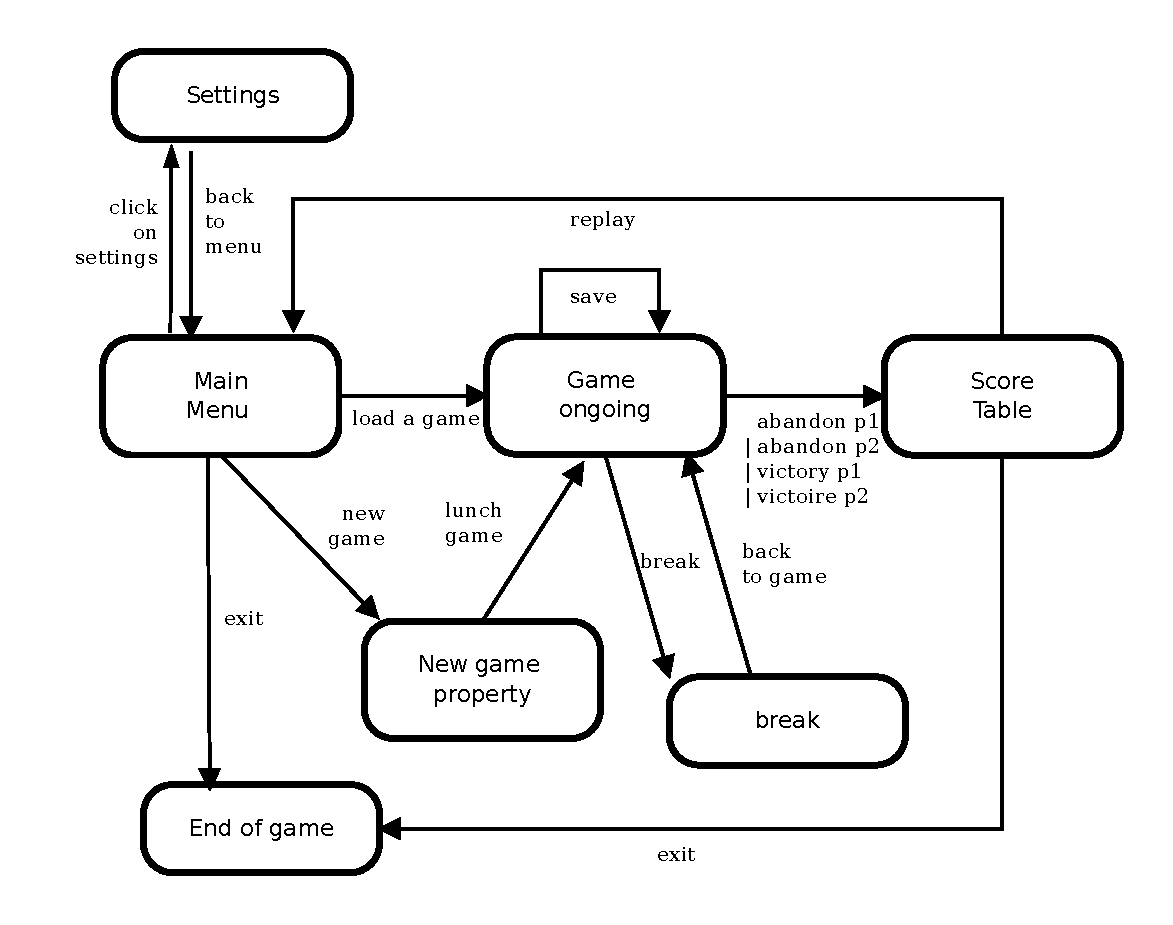
\includegraphics[width=0.7\textwidth]{figure/etat_transition_partie.pdf}
			\end{center}
			\caption{Diagrame d'états-transitions}
			\label{fig:transition_jeu}
		\end{figure}
	
		le diagramme d'état-transition présenter en FIGURE \ref{fig:transition_jeu} présente les différents état dans lequel le programme \emph{Bedbihan} peut se situer, il modélise ainsi les différentes phases du jeu.


		\subsection{Le lancement du jeu}

		Au lancement du jeu, l'utilisateur à le choix entre débuter une nouvelle partie et reprendre une partie préalablement sauvegarder. Le lancement d'une nouvelle partie implique le choix d'une taille de carte, ainsi que le choix d'un peuple pour chacun des joueurs. 

		Ceci est illustré par le diagramme d'utilisation présenté en FIGURE \ref{fig:use1}.

		\begin{figure}
			\begin{center}
				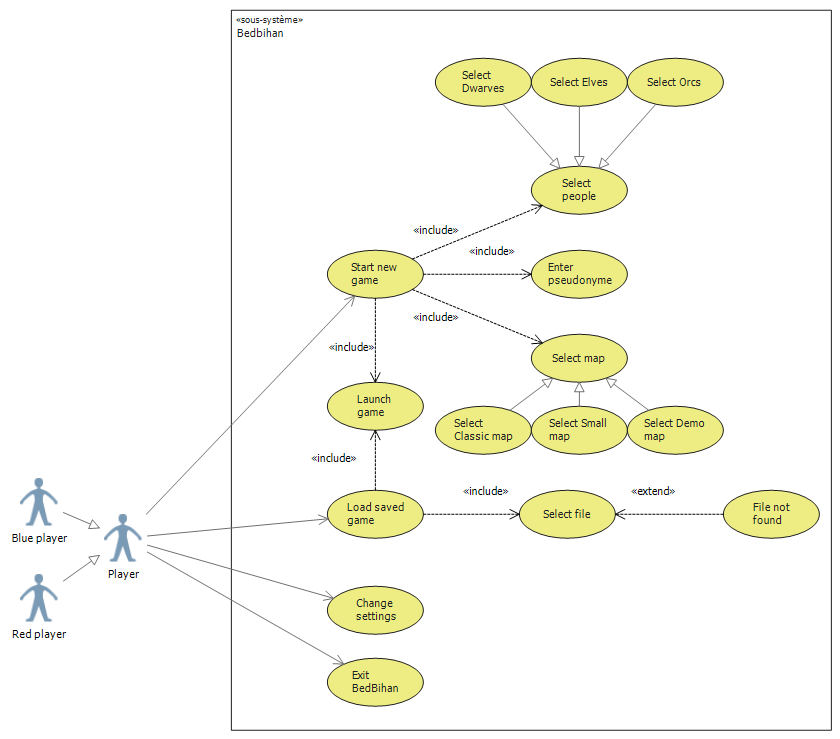
\includegraphics[width=1\textwidth]{figure/cas_utilisation_1.png}
			\end{center}
			\caption{Cas d'utilisation numéro 1}
			\label{fig:use1}
		\end{figure}



	\subsection{le déroulement d'un tour}

		\emph{BedBihan} se joue à tour de rôle. Lors d'un tour le joueur dispose d'un nombre définie d'actions à réaliser. Cela est illusté par le diagramme d'utilisation présenté en FIGURE \ref{fig:use2}.

		\begin{figure}
			\begin{center}
				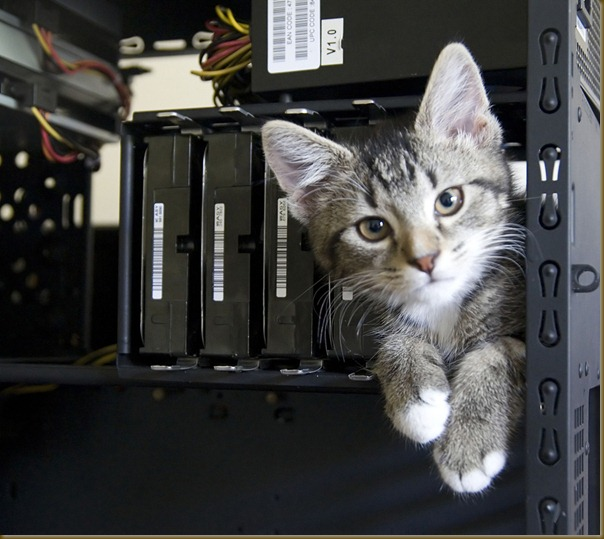
\includegraphics[width=1\textwidth]{figure/cas_utilisation_2.jpg}
			\end{center}
			\caption{Cas d'utilisation numéro 2}
			\label{fig:use2}
		\end{figure}


	\subsection{le déroulement d'un combat}


		Dans \emph{BedBihan}, quand un joueur souhaite déplacer une unité sur une case occupée par une unité enemie, il provoque un combat. 
